% ============================================================================
% APPENDIX B: SCREENSHOTS
% ============================================================================

\chapter{SCREENSHOTS}

This appendix contains screenshots documenting the system's training process, results visualization, and explainability analysis outputs.

\section{Training Output}

\begin{figure}[H]
    \centering
    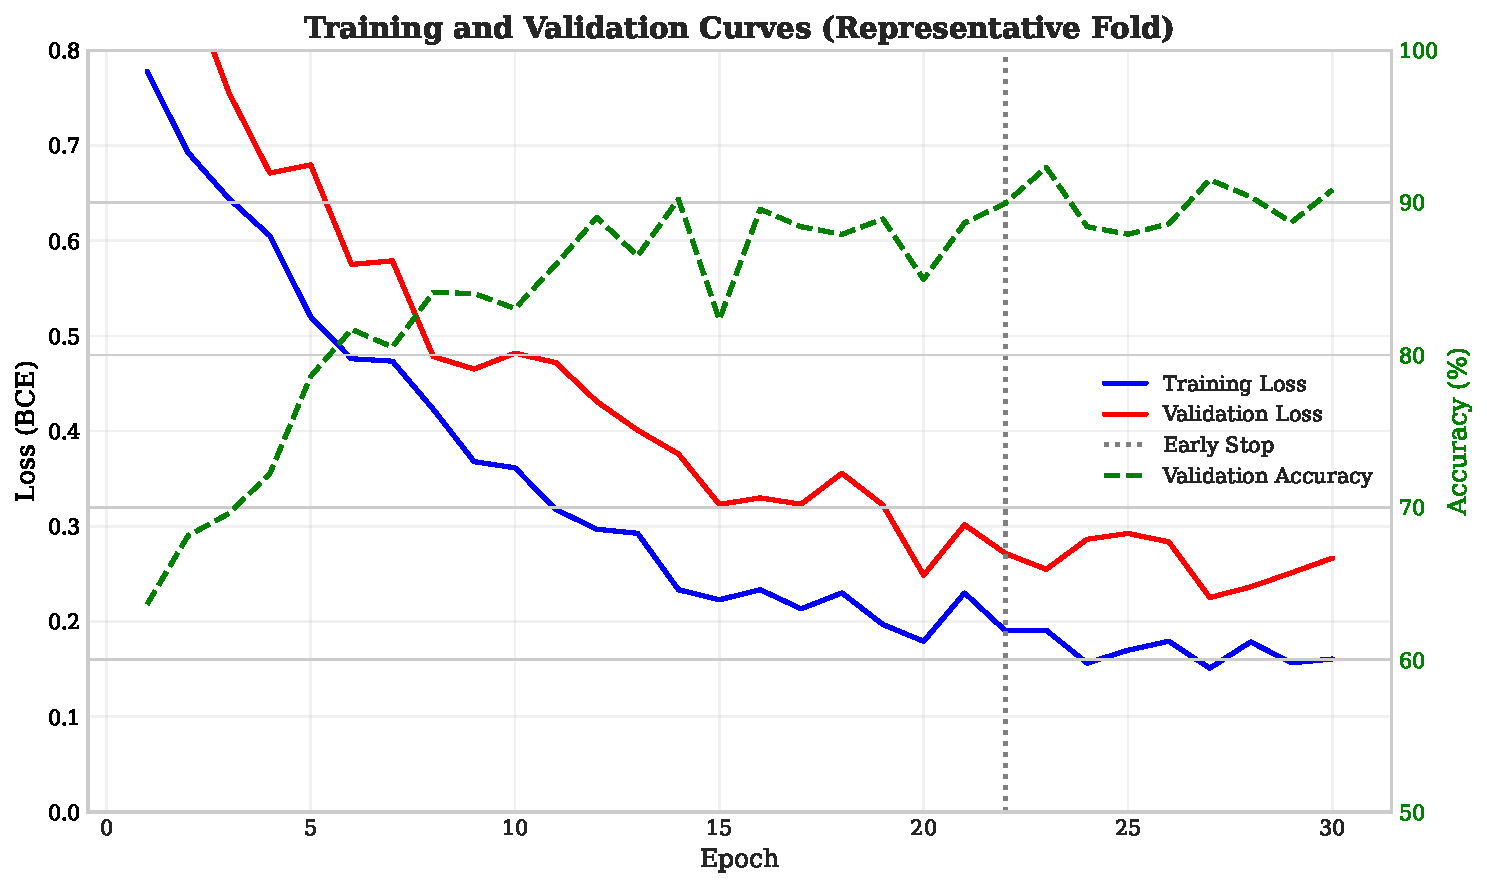
\includegraphics[width=0.9\textwidth]{figures/ch4/fig4_4_training_curves.pdf}
    \caption{Training and validation loss curves showing model convergence over 30 epochs with early stopping based on validation loss.}
    \label{fig:training_output}
\end{figure}

\section{Results Visualization}

\begin{figure}[H]
    \centering
    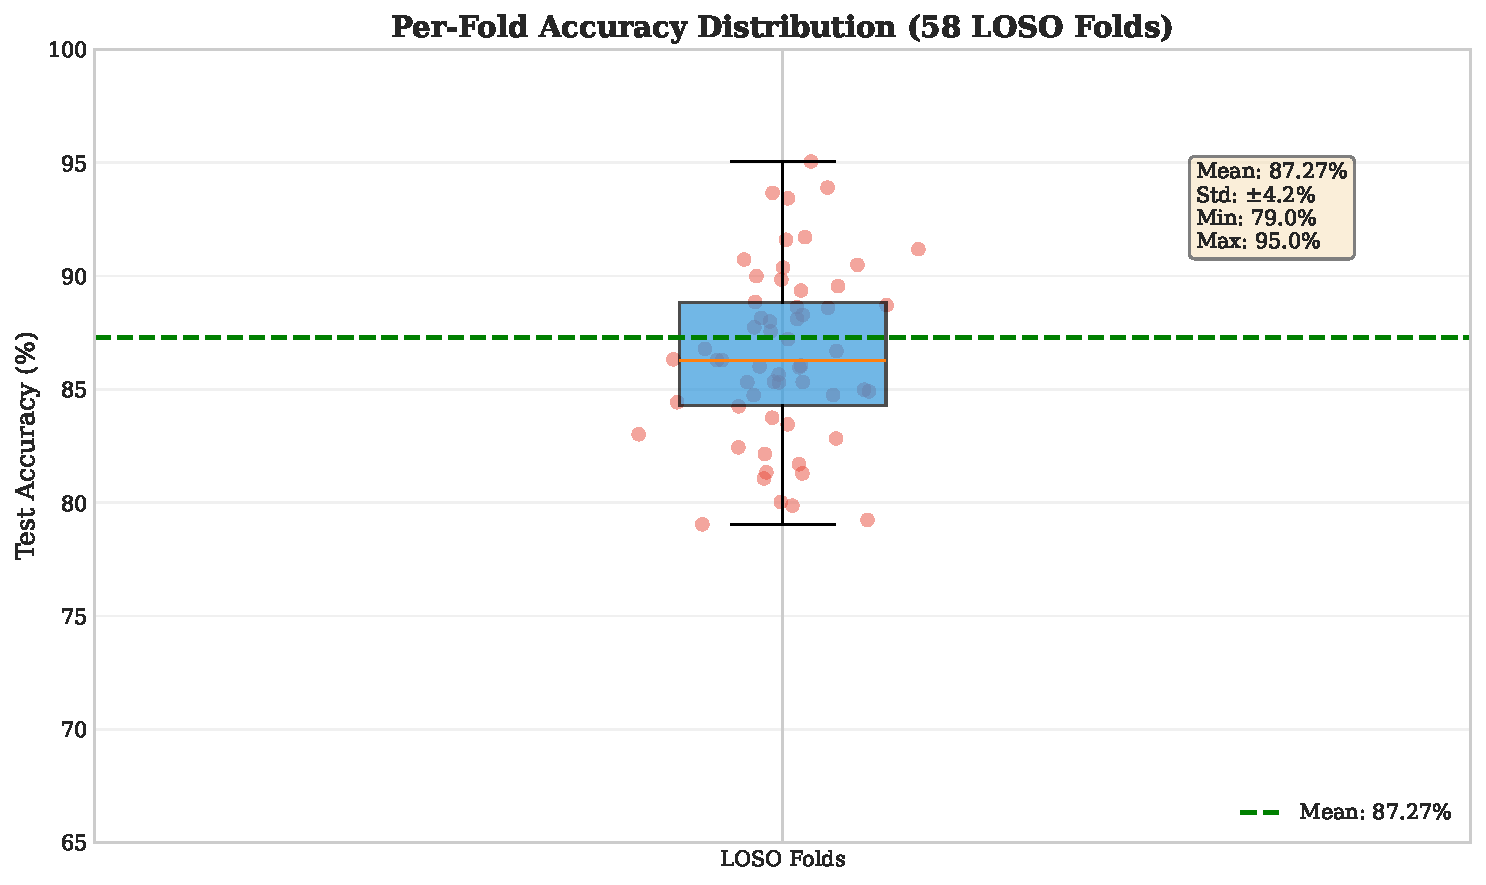
\includegraphics[width=0.85\textwidth]{figures/ch4/fig4_7_fold_distribution.pdf}
    \caption{Distribution of per-fold accuracies across all 58 LOSO cross-validation folds, demonstrating consistent model performance.}
    \label{fig:loss_curves}
\end{figure}

\begin{figure}[H]
    \centering
    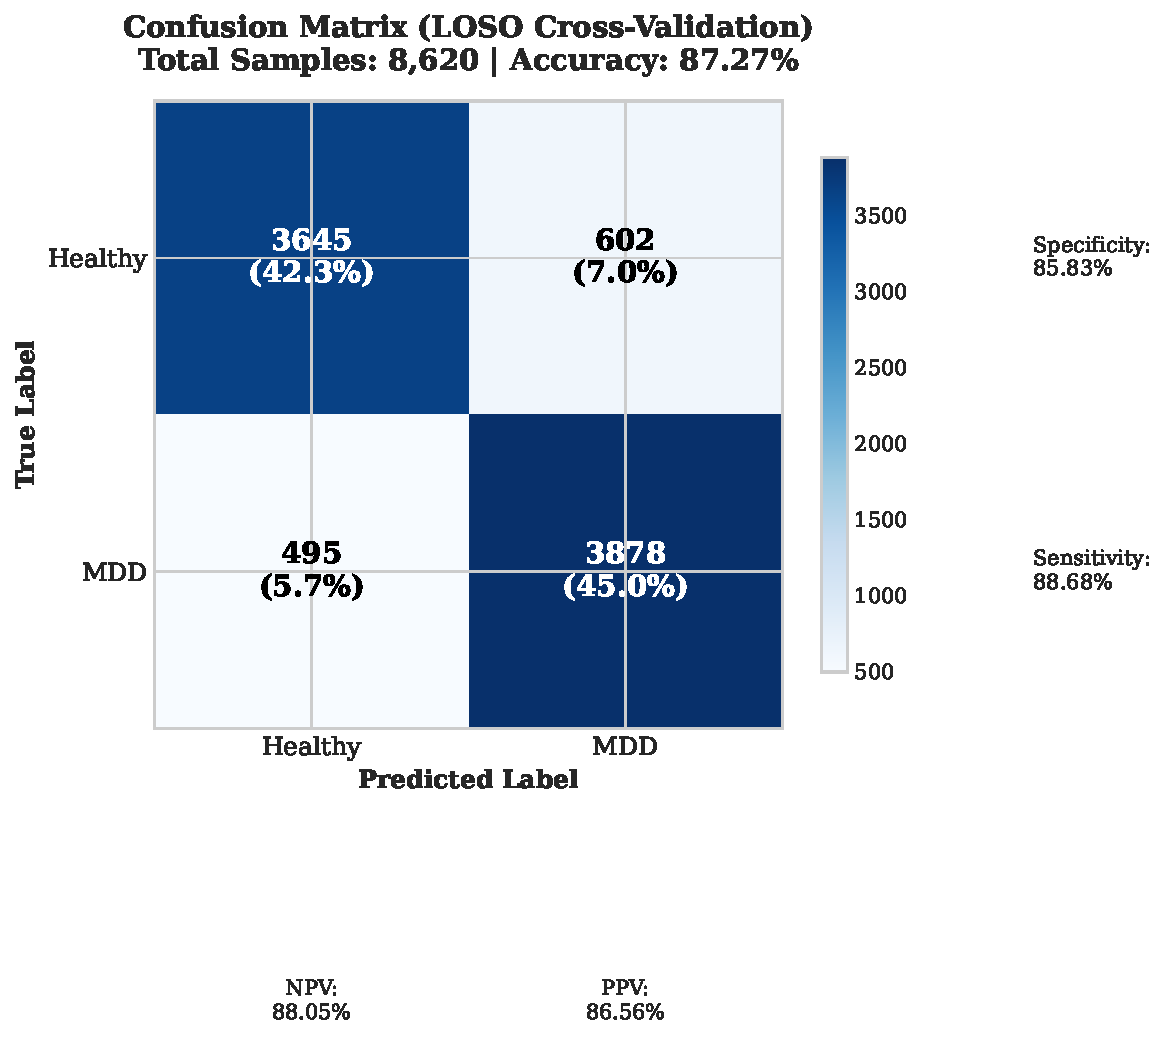
\includegraphics[width=0.85\textwidth]{figures/ch4/fig4_5_confusion_matrix.pdf}
    \caption{Confusion matrix showing the aggregate classification results across all 58 LOSO folds with true positives, true negatives, false positives, and false negatives.}
    \label{fig:per_subject_acc}
\end{figure}

\section{Explainability Visualizations}

\begin{figure}[H]
    \centering
    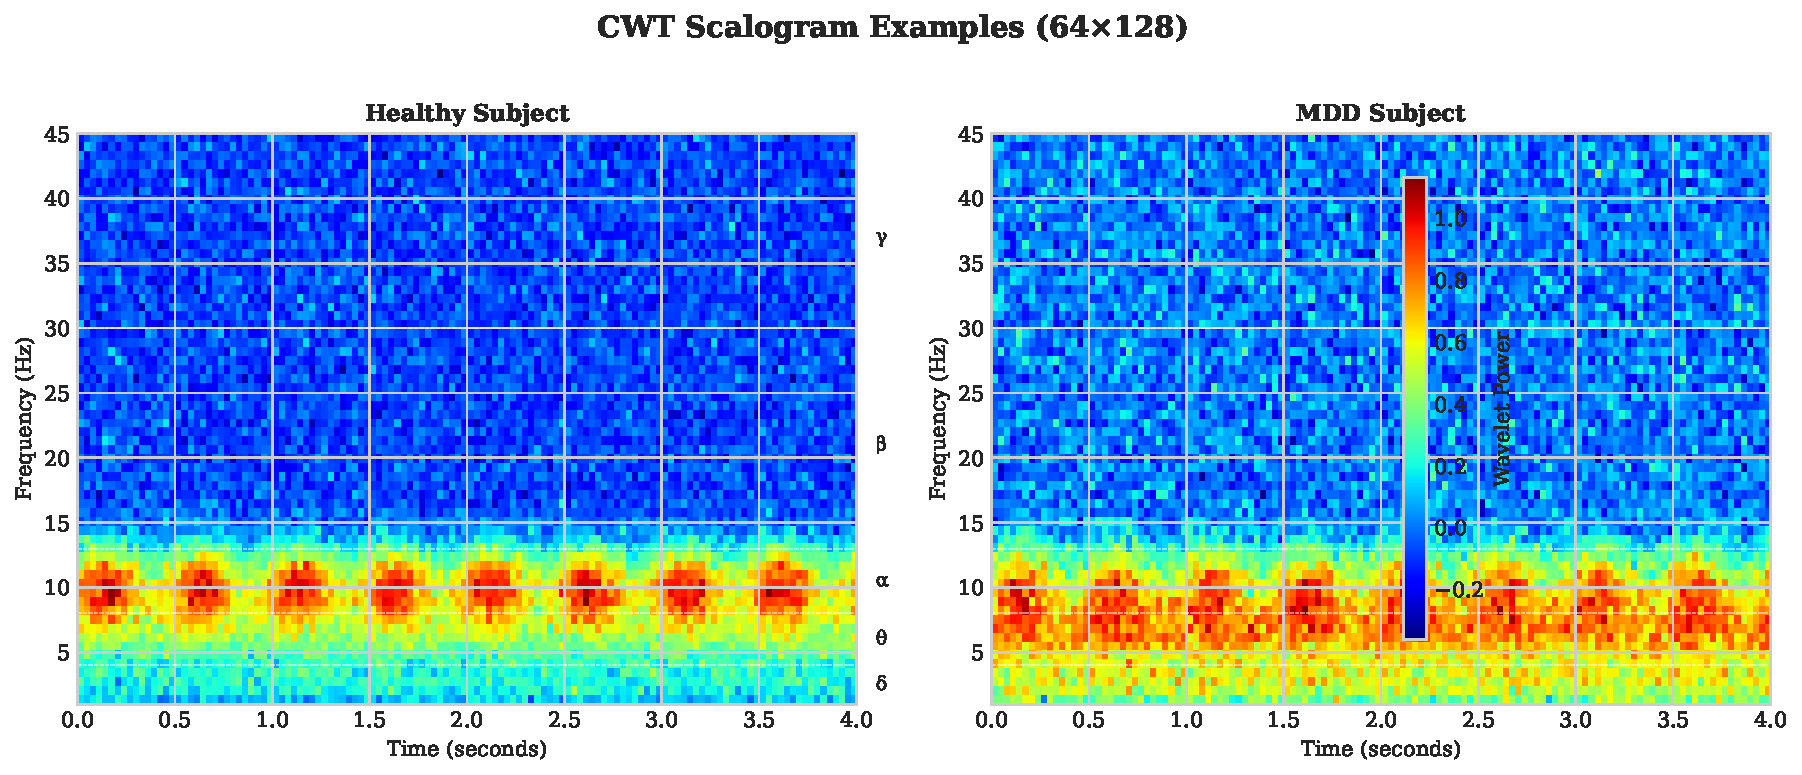
\includegraphics[width=0.85\textwidth]{figures/ch3/fig3_6_cwt_scalogram.pdf}
    \caption{CWT scalogram time-frequency representation used as input to the Transformer branch. The model learns to attend to discriminative frequency bands through Integrated Gradients analysis.}
    \label{fig:ig_attribution}
\end{figure}

\begin{figure}[H]
    \centering
    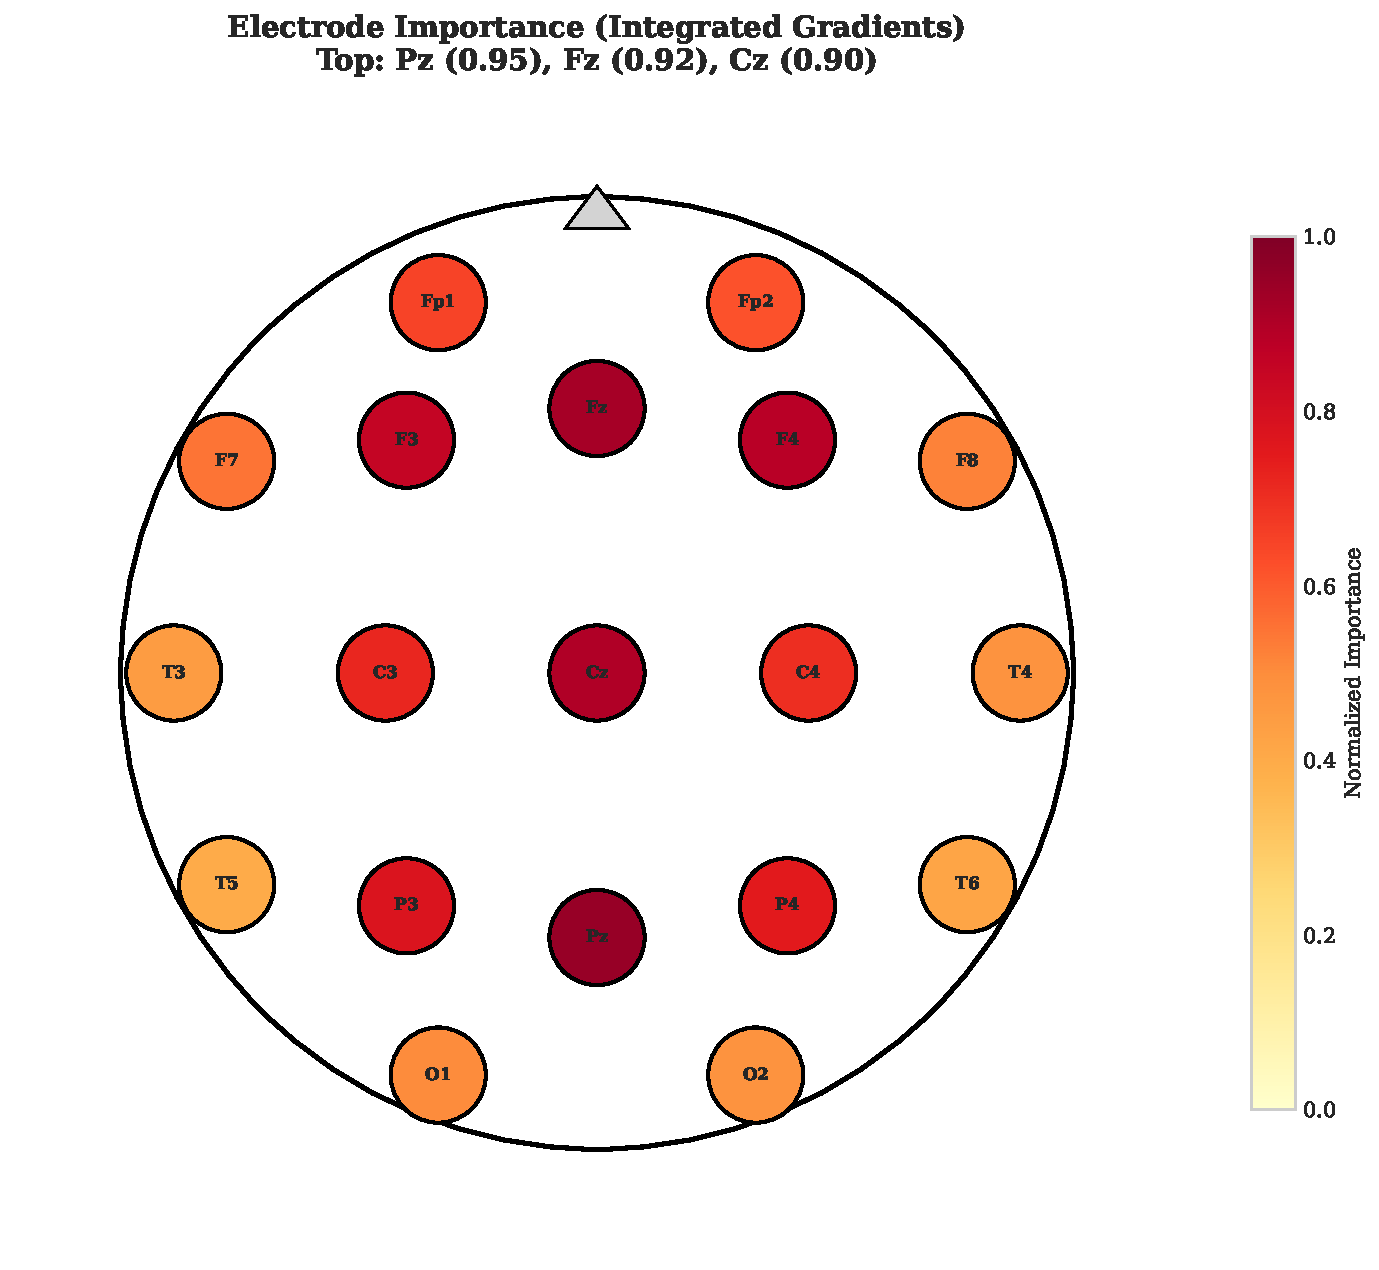
\includegraphics[width=0.75\textwidth]{figures/ch4/fig4_8_electrode_importance.pdf}
    \caption{Topographic map of electrode importance derived from Integrated Gradients analysis, showing frontal electrodes (F3, F4, Fz) with highest contribution to depression classification.}
    \label{fig:topomap}
\end{figure}

\begin{figure}[H]
    \centering
    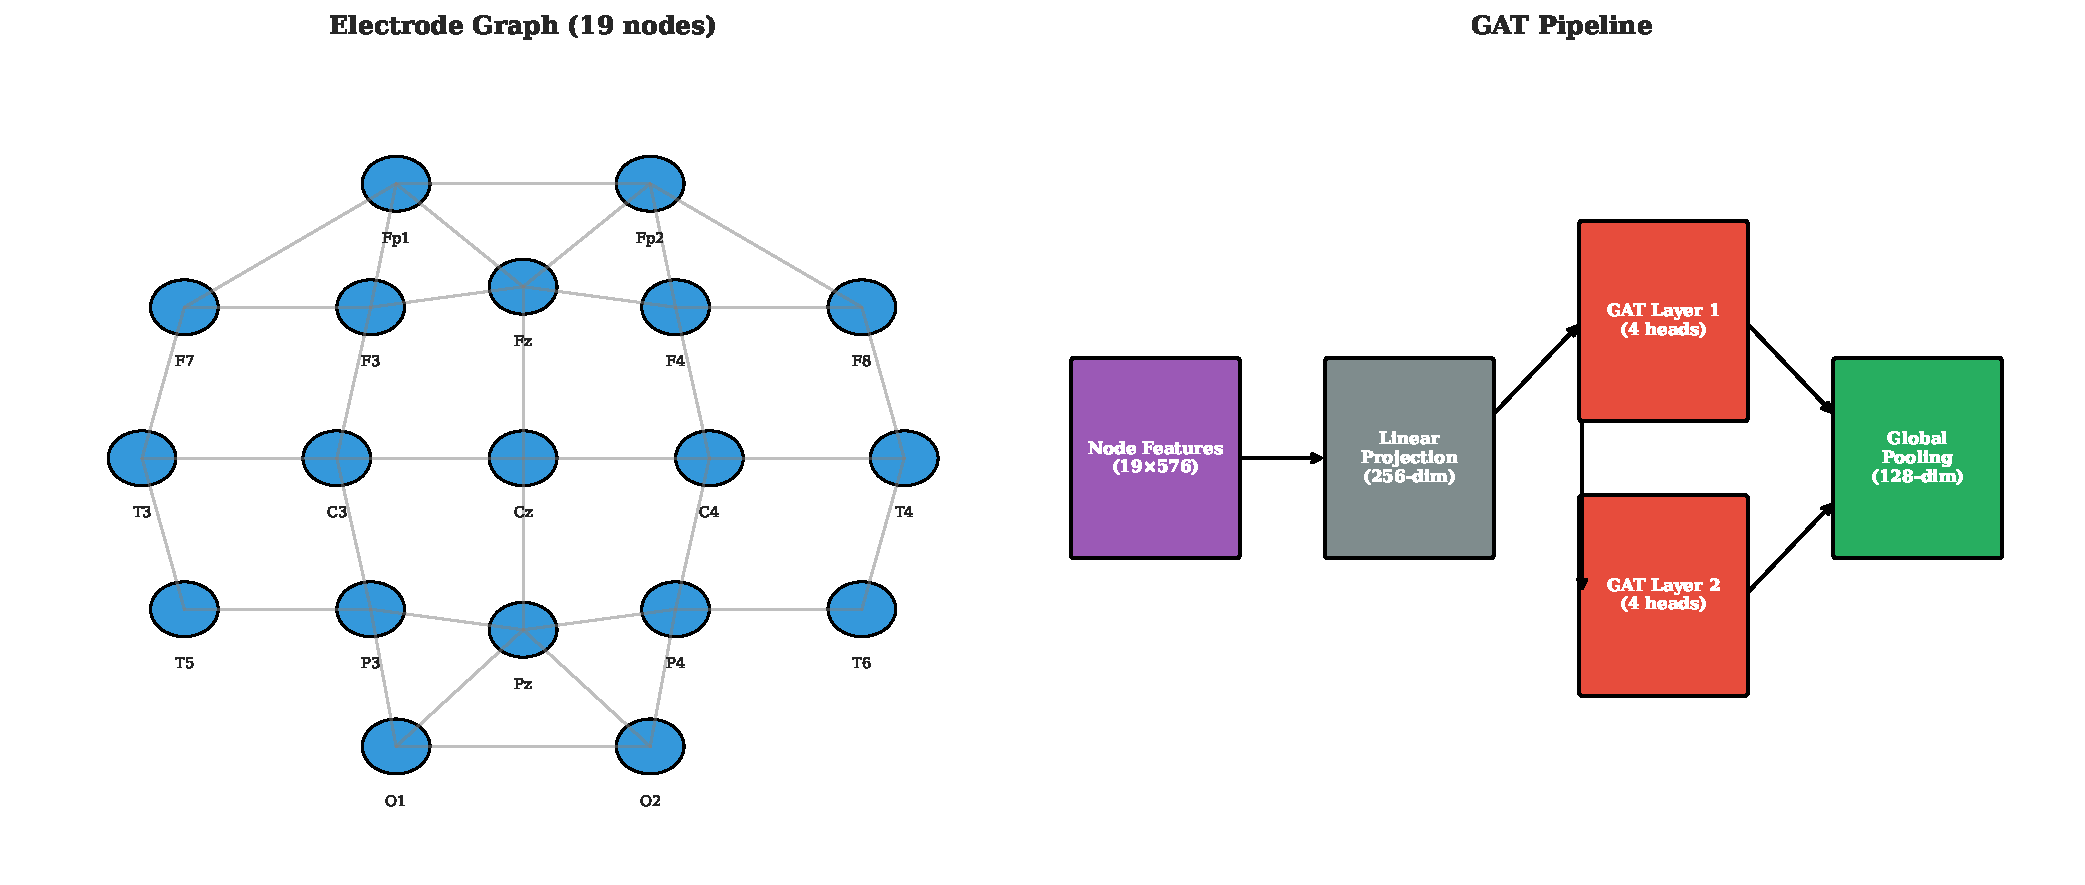
\includegraphics[width=0.85\textwidth]{figures/ch3/fig3_8_gnn.pdf}
    \caption{GNN architecture showing electrode graph construction with 19 nodes representing EEG channels and learned attention-weighted connections between electrodes.}
    \label{fig:gnn_attention}
\end{figure}

\section{Model Architecture Visualization}

\begin{figure}[H]
    \centering
    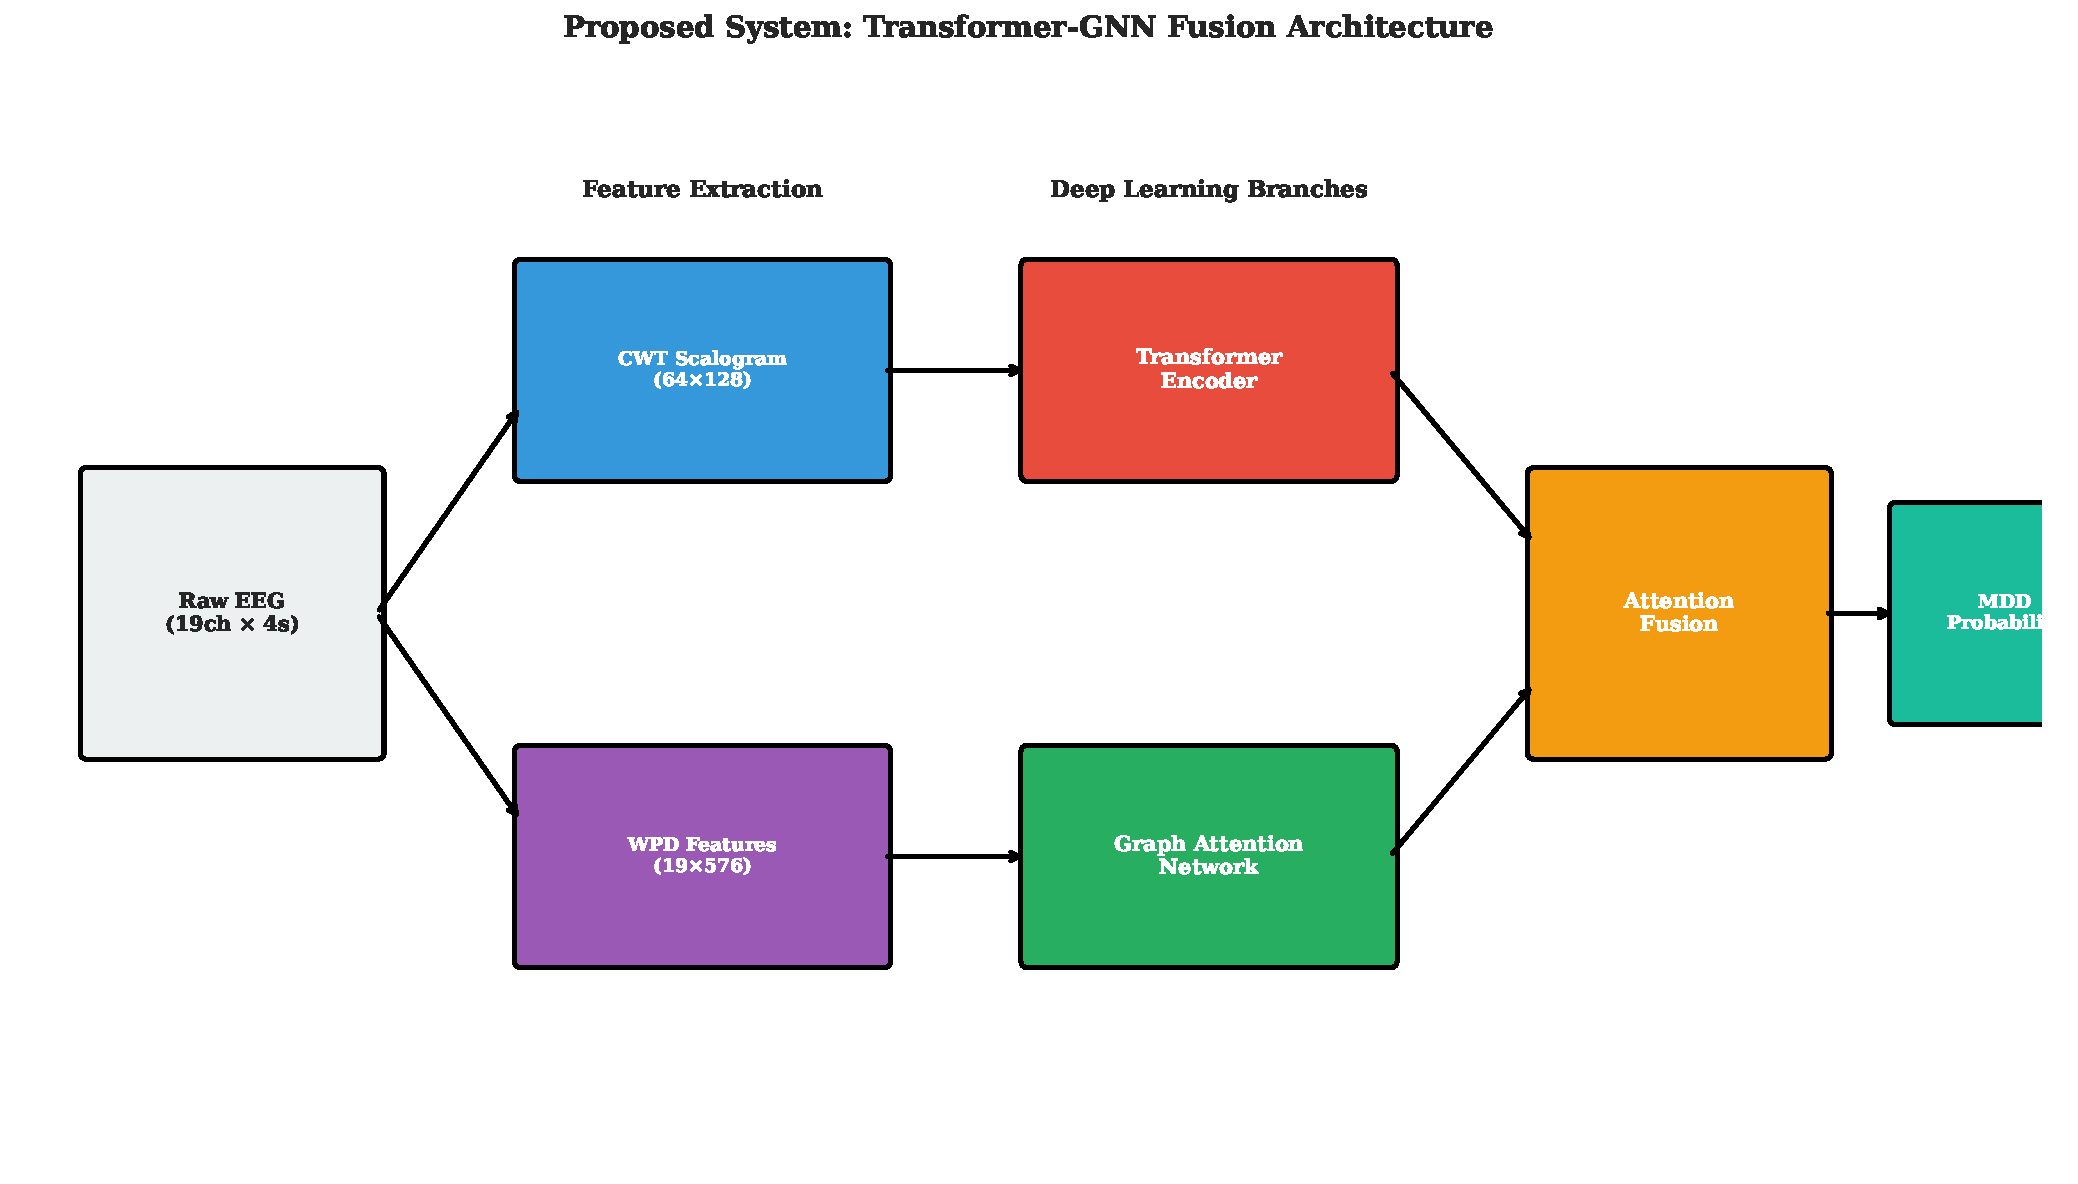
\includegraphics[width=0.95\textwidth]{figures/ch2/fig2_4_proposed_architecture.pdf}
    \caption{Complete model architecture showing the dual-branch design with Transformer processing CWT scalograms and GNN processing WPD features, followed by attention-based fusion and classification.}
    \label{fig:model_graph}
\end{figure}

\section{Sample Predictions}

\begin{figure}[H]
    \centering
    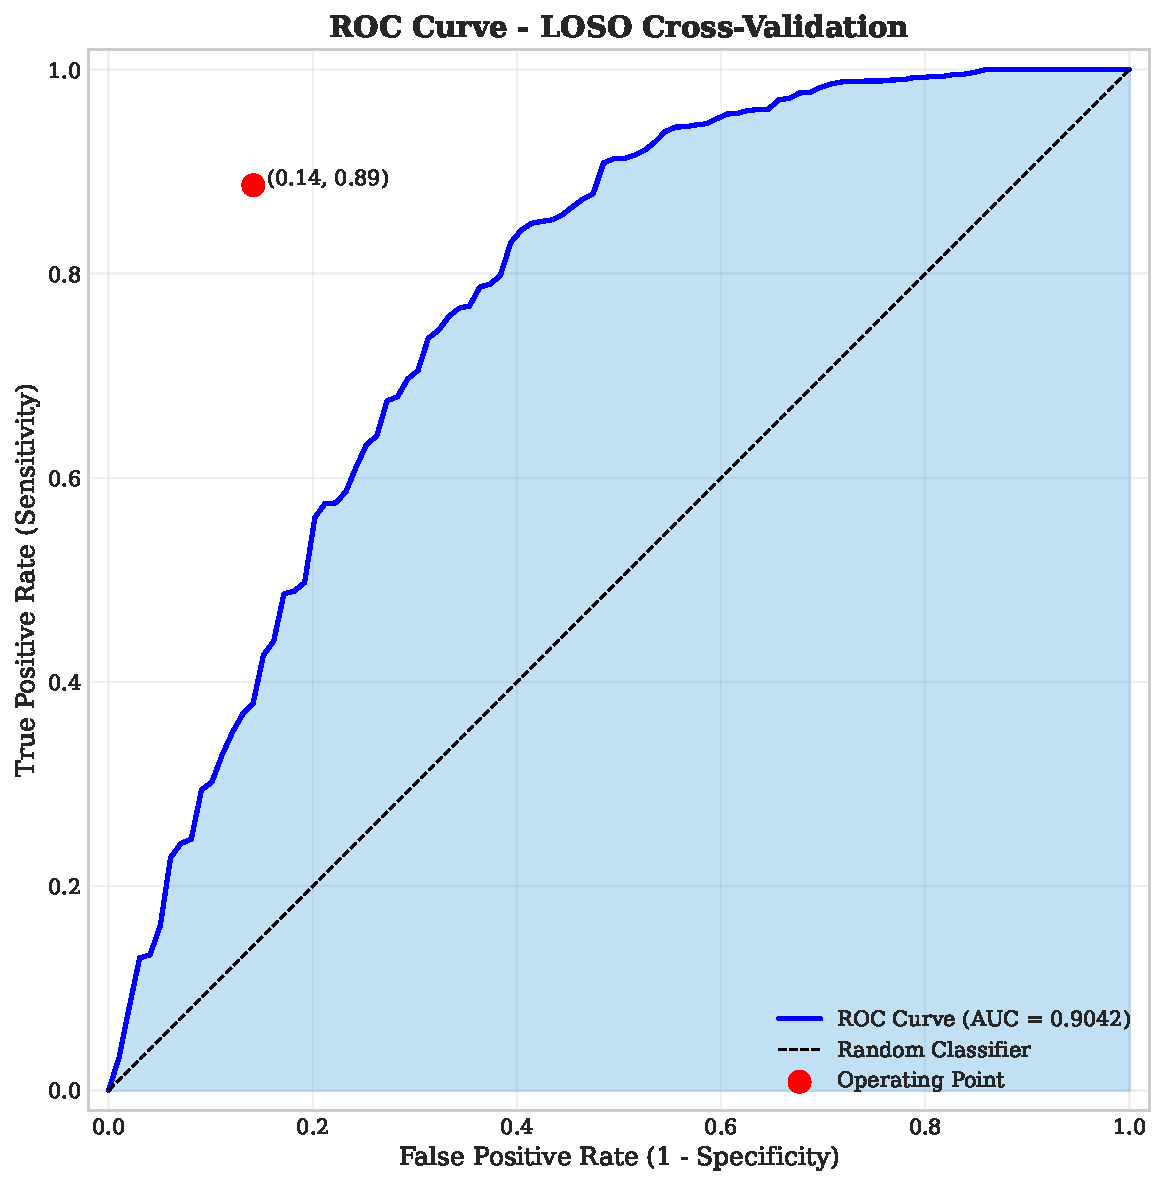
\includegraphics[width=0.85\textwidth]{figures/ch4/fig4_6_roc_curve.pdf}
    \caption{ROC curve analysis showing model discrimination capability across different classification thresholds, with AUC = 0.9042 indicating excellent performance.}
    \label{fig:sample_predictions}
\end{figure}

\section{Project Directory Structure}

\begin{lstlisting}[language=bash, caption={Project Directory Tree}]
eeg_depression_detection/
|-- config/
|   |-- data_config.yaml
|   |-- model_config.yaml
|   `-- training_config.yaml
|-- data/
|   |-- datasets/
|   |   `-- figshare_dataset.py
|   |-- preprocessing/
|   |   `-- filters.py
|   `-- raw/figshare/
|       `-- cache/
|-- features/
|   `-- wavelet/
|       |-- cwt_extractor.py
|       `-- wpd_extractor.py
|-- models/
|   |-- branches/
|   |   |-- bilstm_encoder.py
|   |   |-- gnn_encoder.py
|   |   `-- transformer_encoder.py
|   |-- fusion/
|   |   |-- attention_fusion.py
|   |   `-- three_way_fusion.py
|   |-- full_model.py
|   `-- full_model_v2.py
|-- training/
|   `-- trainer.py
|-- scripts/
|   |-- train.py
|   |-- train_v2.py
|   `-- train_v2_parallel.py
|-- explainability/
|   |-- integrated_gradients.py
|   |-- lrp.py
|   |-- tcav.py
|   |-- run_explainability.py
|   `-- run_explainability_v2.py
|-- outputs/
|   `-- run_20260201_014750/
|       |-- config.json
|       `-- results.json
|-- docs/
|   |-- COMPREHENSIVE_PROJECT_REPORT.md
|   |-- EXPLAINABILITY_METHODS.md
|   |-- PROJECT_LOG.md
|   `-- RESEARCH_PAPER_DRAFT.md
|-- requirements.txt
`-- RESEARCH_DOCUMENTATION.md
\end{lstlisting}
